\documentclass{standalone}
\usepackage{tikz}
\usetikzlibrary{shapes.geometric}
\usetikzlibrary{patterns, positioning}
\usetikzlibrary{shapes.misc}
\usepackage[outline]{contour}
\contourlength{1.5pt} 


\begin{document}
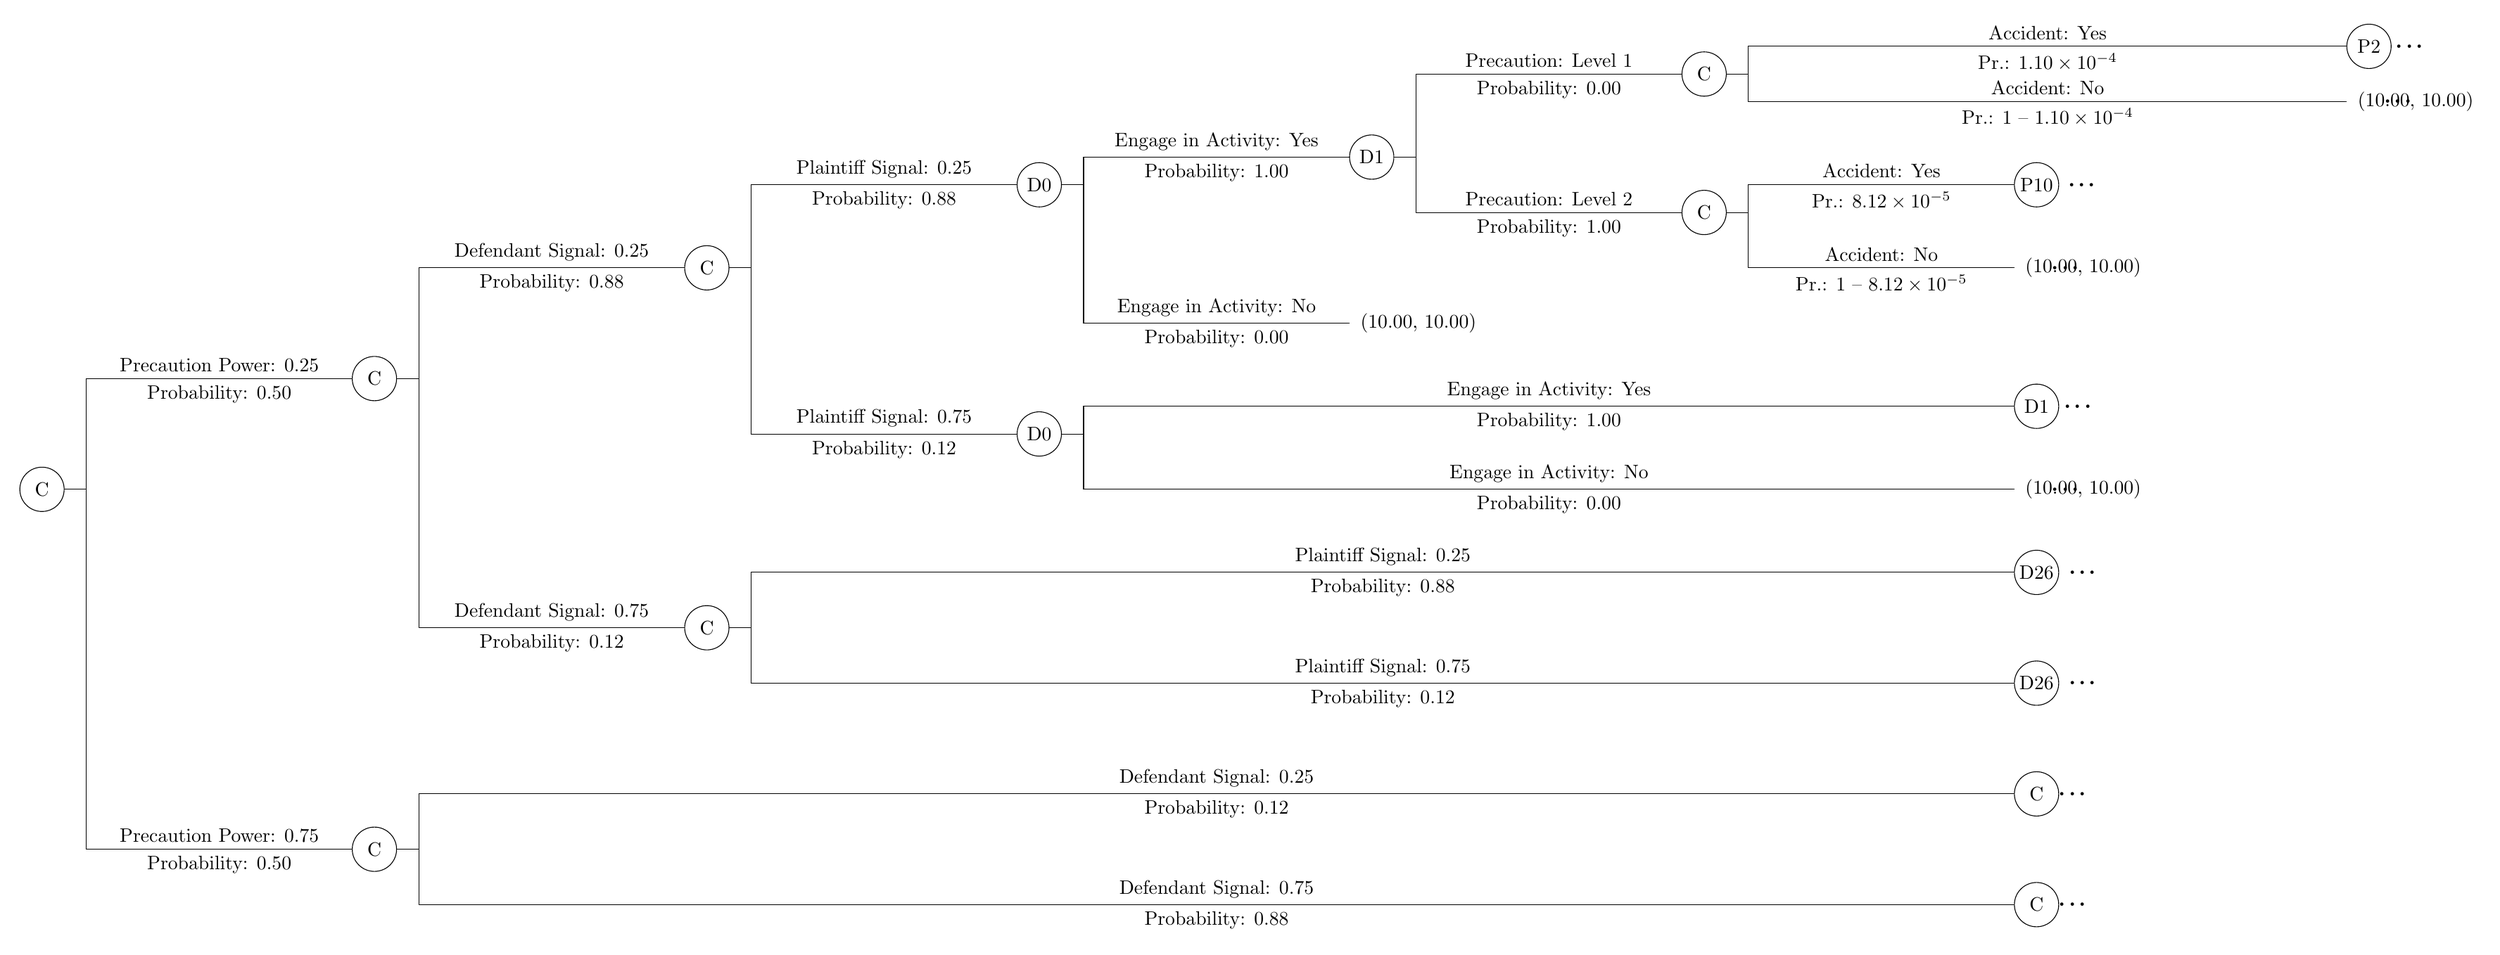
\begin{tikzpicture}

    \draw[color=black] (-42, -8.25) circle (0.4cm) node[draw=none] (N0) {C};

    \draw[color=black] (-36, -6.25) circle (0.4cm) node[draw=none] (N0) {C};
\draw (-41.6, -8.25) -- (-41.2, -8.25) -- (-41.2, -6.25) -- (-36.4, -6.25) node [midway, above, sloped] (E0) {Precaution Power: 0.25} node [midway, below, sloped] (E1) {Probability: 0.50} ;


    \draw[color=black] (-30, -4.25) circle (0.4cm) node[draw=none] (N2) {C};
\draw (-35.6, -6.25) -- (-35.2, -6.25) -- (-35.2, -4.25) -- (-30.4, -4.25) node [midway, above, sloped] (E2) {Defendant Signal: 0.25} node [midway, below, sloped] (E3) {Probability: 0.88} ;


    \draw[color=black] (-24, -2.75) circle (0.4cm) node[draw=none] (N4) {D0};
\draw (-29.6, -4.25) -- (-29.200000000000003, -4.25) -- (-29.200000000000003, -2.75) -- (-24.4, -2.75) node [midway, above, sloped] (E4) {Plaintiff Signal: 0.25} node [midway, below, sloped] (E5) {Probability: 0.88} ;


    \draw[color=black] (-18, -2.25) circle (0.4cm) node[draw=none] (N6) {D1};
\draw (-23.6, -2.75) -- (-23.200000000000003, -2.75) -- (-23.200000000000003, -2.25) -- (-18.4, -2.25) node [midway, above, sloped] (E6) {Engage in Activity: Yes} node [midway, below, sloped] (E7) {Probability: 1.00} ;


    \draw[color=black] (-12, -0.75) circle (0.4cm) node[draw=none] (N8) {C};
\draw (-17.6, -2.25) -- (-17.200000000000003, -2.25) -- (-17.200000000000003, -0.75) -- (-12.4, -0.75) node [midway, above, sloped] (E8) {Precaution: Level 1} node [midway, below, sloped] (E9) {Probability: 0.00} ;


    \draw[color=black] (0, -0.25) circle (0.4cm) node[draw=none] (N10) {P2};
\node[draw=none, right=0cm of N10,font=\huge] {...};
\draw (-11.6, -0.75) -- (-11.2, -0.75) -- (-11.2, -0.25) -- (-0.4, -0.25) node [midway, above, sloped] (E10) {Accident: Yes} node [midway, below, sloped] (E11) {Pr.: $1.10 \times 10^{-4}$} ;


    \draw[color=black] (0, -1.25) node[draw=none] (N12) {};
\node[draw=none, right=-0.45cm of N12] {(10.00, 10.00)};
\node[draw=none, right=0cm of N12,font=\huge] {...};
\draw (-11.6, -0.75) -- (-11.2, -0.75) -- (-11.2, -1.25) -- (-0.4, -1.25) node [midway, above, sloped] (E12) {Accident: No} node [midway, below, sloped] (E13) {Pr.: 1 -- $1.10 \times 10^{-4}$} ;


    \draw[color=black] (-12, -3.25) circle (0.4cm) node[draw=none] (N14) {C};
\draw (-17.6, -2.25) -- (-17.200000000000003, -2.25) -- (-17.200000000000003, -3.25) -- (-12.4, -3.25) node [midway, above, sloped] (E14) {Precaution: Level 2} node [midway, below, sloped] (E15) {Probability: 1.00} ;


    \draw[color=black] (-6, -2.75) circle (0.4cm) node[draw=none] (N16) {P10};
\node[draw=none, right=0cm of N16,font=\huge] {...};
\draw (-11.6, -3.25) -- (-11.2, -3.25) -- (-11.2, -2.75) -- (-6.4, -2.75) node [midway, above, sloped] (E16) {Accident: Yes} node [midway, below, sloped] (E17) {Pr.: $8.12 \times 10^{-5}$} ;


    \draw[color=black] (-6, -4.25) node[draw=none] (N18) {};
\node[draw=none, right=-0.45cm of N18] {(10.00, 10.00)};
\node[draw=none, right=0cm of N18,font=\huge] {...};
\draw (-11.6, -3.25) -- (-11.2, -3.25) -- (-11.2, -4.25) -- (-6.4, -4.25) node [midway, above, sloped] (E18) {Accident: No} node [midway, below, sloped] (E19) {Pr.: 1 -- $8.12 \times 10^{-5}$} ;


    \draw[color=black] (-18, -5.25) node[draw=none] (N20) {};
\node[draw=none, right=-0.45cm of N20] {(10.00, 10.00)};
\draw (-23.6, -2.75) -- (-23.200000000000003, -2.75) -- (-23.200000000000003, -5.25) -- (-18.4, -5.25) node [midway, above, sloped] (E20) {Engage in Activity: No} node [midway, below, sloped] (E21) {Probability: 0.00} ;


    \draw[color=black] (-24, -7.25) circle (0.4cm) node[draw=none] (N22) {D0};
\draw (-29.6, -4.25) -- (-29.200000000000003, -4.25) -- (-29.200000000000003, -7.25) -- (-24.4, -7.25) node [midway, above, sloped] (E22) {Plaintiff Signal: 0.75} node [midway, below, sloped] (E23) {Probability: 0.12} ;


    \draw[color=black] (-6, -6.75) circle (0.4cm) node[draw=none] (N24) {D1};
\node[draw=none, right=0cm of N24,font=\huge] {...};
\draw (-23.6, -7.25) -- (-23.200000000000003, -7.25) -- (-23.200000000000003, -6.75) -- (-6.4, -6.75) node [midway, above, sloped] (E24) {Engage in Activity: Yes} node [midway, below, sloped] (E25) {Probability: 1.00} ;


    \draw[color=black] (-6, -8.25) node[draw=none] (N26) {};
\node[draw=none, right=-0.45cm of N26] {(10.00, 10.00)};
\node[draw=none, right=0cm of N26,font=\huge] {...};
\draw (-23.6, -7.25) -- (-23.200000000000003, -7.25) -- (-23.200000000000003, -8.25) -- (-6.4, -8.25) node [midway, above, sloped] (E26) {Engage in Activity: No} node [midway, below, sloped] (E27) {Probability: 0.00} ;


    \draw[color=black] (-30, -10.75) circle (0.4cm) node[draw=none] (N28) {C};
\draw (-35.6, -6.25) -- (-35.2, -6.25) -- (-35.2, -10.75) -- (-30.4, -10.75) node [midway, above, sloped] (E28) {Defendant Signal: 0.75} node [midway, below, sloped] (E29) {Probability: 0.12} ;


    \draw[color=black] (-6, -9.75) circle (0.4cm) node[draw=none] (N30) {D26};
\node[draw=none, right=0cm of N30,font=\huge] {...};
\draw (-29.6, -10.75) -- (-29.200000000000003, -10.75) -- (-29.200000000000003, -9.75) -- (-6.4, -9.75) node [midway, above, sloped] (E30) {Plaintiff Signal: 0.25} node [midway, below, sloped] (E31) {Probability: 0.88} ;


    \draw[color=black] (-6, -11.75) circle (0.4cm) node[draw=none] (N32) {D26};
\node[draw=none, right=0cm of N32,font=\huge] {...};
\draw (-29.6, -10.75) -- (-29.200000000000003, -10.75) -- (-29.200000000000003, -11.75) -- (-6.4, -11.75) node [midway, above, sloped] (E32) {Plaintiff Signal: 0.75} node [midway, below, sloped] (E33) {Probability: 0.12} ;


    \draw[color=black] (-36, -14.75) circle (0.4cm) node[draw=none] (N34) {C};
\draw (-41.6, -8.25) -- (-41.2, -8.25) -- (-41.2, -14.75) -- (-36.4, -14.75) node [midway, above, sloped] (E34) {Precaution Power: 0.75} node [midway, below, sloped] (E35) {Probability: 0.50} ;


    \draw[color=black] (-6, -13.75) circle (0.4cm) node[draw=none] (N36) {C};
\node[draw=none, right=0cm of N36,font=\huge] {...};
\draw (-35.6, -14.75) -- (-35.2, -14.75) -- (-35.2, -13.75) -- (-6.4, -13.75) node [midway, above, sloped] (E36) {Defendant Signal: 0.25} node [midway, below, sloped] (E37) {Probability: 0.12} ;


    \draw[color=black] (-6, -15.75) circle (0.4cm) node[draw=none] (N38) {C};
\node[draw=none, right=0cm of N38,font=\huge] {...};
\draw (-35.6, -14.75) -- (-35.2, -14.75) -- (-35.2, -15.75) -- (-6.4, -15.75) node [midway, above, sloped] (E38) {Defendant Signal: 0.75} node [midway, below, sloped] (E39) {Probability: 0.88} ;


\end{tikzpicture}
\end{document}